\documentclass[11pt]{article}
\addtolength{\oddsidemargin}{-1.cm}
\addtolength{\textwidth}{2cm}
\addtolength{\topmargin}{-2cm}
\addtolength{\textheight}{3.5cm}

\usepackage[pdftex]{graphicx}
\usepackage{hyperref}
\usepackage{cleveref}
\usepackage{float}
\usepackage{cite}
\usepackage{placeins}
\usepackage{booktabs}
\hypersetup{
	colorlinks=true,
	linkcolor=black,
	filecolor=magenta,
	urlcolor=cyan,
}

% define the title
\author{Team CodeX}
\title{User Manual}

\begin{document}
	\setcounter{tocdepth}{6}
	\setcounter{secnumdepth}{6}
	\setlength{\parskip}{6pt}
	
	% generates the title
	\begin{titlepage}
	
	\begin{center}
		% Upper part of the page       
		
\includegraphics[width=0.7\linewidth]{../Images/eVoting_Logo.png}\\[2cm]    
		\textsc{\LARGE Electronic Voting}\\[0.5cm]
		% Title
		\rule{\linewidth}{0.5mm} \\[1cm]
		{ \huge \bfseries User Manual}\\[0.5cm]
		\rule{\linewidth}{0.5mm} \\[1cm]
		
		% Author and supervisor
<<<<<<< HEAD
		
\includegraphics[width=0.5\linewidth]{../Images/TeamCodexLogo.jpg}\\[0.5cm]    	
=======
		
		
\includegraphics[width=0.5\textwidth]{../Images/TeamCodexLogo.jpg}\\[0.5cm]    	
>>>>>>> 9b25dd959830e00c0e449a84c7623c3e326c347b
		
		
		\begin{minipage}{0.4\textwidth}
			\begin{flushleft} \large
				Andreas {du Preez}
			\end{flushleft}
		\end{minipage}
		\begin{minipage}{0.4\textwidth}
			\begin{flushright} \large
				\emph{} \\
				12207871 
			\end{flushright}
		\end{minipage}
		
		
		\begin{minipage}{0.4\textwidth}
			\begin{flushleft} \large
				\emph{} \\
				Azhar {Mohungoo }
			\end{flushleft}
		\end{minipage}
		\begin{minipage}{0.4\textwidth}
			\begin{flushright} \large
				\emph{} \\
				12239799
			\end{flushright}
		\end{minipage}
		
		
		\begin{minipage}{0.4\textwidth}
			\begin{flushleft} \large
				\emph{} \\
				Gift {Sefako }
			\end{flushleft}
		\end{minipage}
		\begin{minipage}{0.4\textwidth}
			\begin{flushright} \large
				\emph{} \\
				12231097
			\end{flushright}
		\end{minipage}
		
		\textsc{\Large Stakeholders}\\[1cm]	
				
		\begin{minipage}{0.4\textwidth}
			\begin{flushleft} \large
				\emph{} \\
				Epi-Use Advance
			\end{flushleft}
		\end{minipage}
		\begin{minipage}{0.4\textwidth}
			\begin{flushright} \large
				\emph{} \\
				Roelof Nuade
			\end{flushright}
		\end{minipage}
		
	\end{center}
\end{titlepage}
	
	\renewcommand{\thesection}{\arabic{section}}
	\newpage
	
	\tableofcontents
	
	\textsc{}\\[1cm]
	
	\newpage
	\section{General Information}
	\subsection{System Overview}
	Electronic Voting, or eVoting for short, is a system which does exactly what the name suggest. It allows members of a demographic country to vote for a political party during an election period. It does so that each vote is completely anonymous by using Blockchain technology.\newline\newline
	The system is usable via an online web page and an Android(4.4+) application.\newline\newline
	There are essentially 4 types of users: An Administrator, a Political Party, an Activator and a Voter. Each having their own dedicated functionality. An administrator user can add a political party user, add an activator user, and deactivate a voter account. A political party account can only check the number of votes they currently have. An activator can only activate a user. And a voter can cast votes.\newline\newline
	In order to make Electronic Voting safe and trustworthy, the activator user is needed. Initially when a new user is registered, they will automatically be 'deactivated', which prevents them from casting any type of vote. This is to prevent a voter from creating a bunch of fake accounts and using those fake accounts to vote multiple times. An activator first need to verify the identity of a voter by providing proof of identity (a drivers license or ID document), after which a voter is then activated and will be granted 2 votes: one vote for a national party, and one vote for a provintial party.\newline\newline
	If a user has not registered yet, they can do so on the web site or on the Android application. Apon registration, the user need to provide: a valid ID number, a password used to log into the system, a name, a surname, the location their registered in (pre defined list of values eg. Pretoria, Johannesburg etc), a mobile number and an email address. A voter is the only user type that can register itself, an activator, political party and administrator can only be added by an existing administrator.\newline\newline
	The beautifull part of eVoting is that it uses Blockchain technology, the same technology used in the famous Bitcoin currency. A blockchain is a distributed database that maintains a continuously-growing list of records called blocks secured from tampering and revision. A more indepth description is beyond the scope of this document.
	
	\subsection{System Configuration}
	eVoting can be generaly simplified by Figure \ref{fig:overview}. When a client uses the system, they will communicate with eVoting through a RESTfull webservice, sending an receiving JSON objects. The webservice is connected to a backend, processing the requests which communicate with the database and blockchain. Since the system uses a webservice as a communication medium between the client and backend, it allows possible future expansion of eVoting for example integration of any third party company, or other mobile platforms.
					\begin{figure}[H]
						\centering
						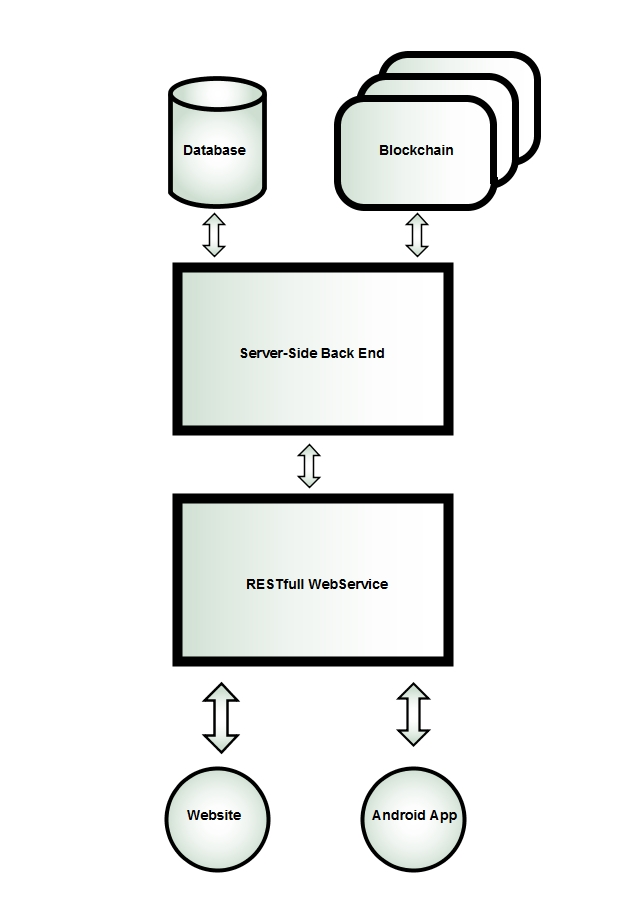
\includegraphics[width=0.75\linewidth]{../Images/UserManual/SystemConfiguration1.jpg}
						\caption{Overview of eVoting}
						\label{fig:overview}
					\end{figure}
					
	The blockchain structure of eVoting is depicted by Figure \ref{fig:blockchainconfig}. It consist of 3 types of nodes: a Root (admin) node, Political Party Node and a Voting Station node. Each of them have different permissions. The Root node has all of the permissions, a Political Party node only has connect and receive permissions and a Voting Station node has connect, send, receive and mine permissions. It is important to keep the eVoting blockchain private from public usage, so new nodes must be approved and added by the root node explicitly.
	\newline
	
						\begin{figure}[H]
							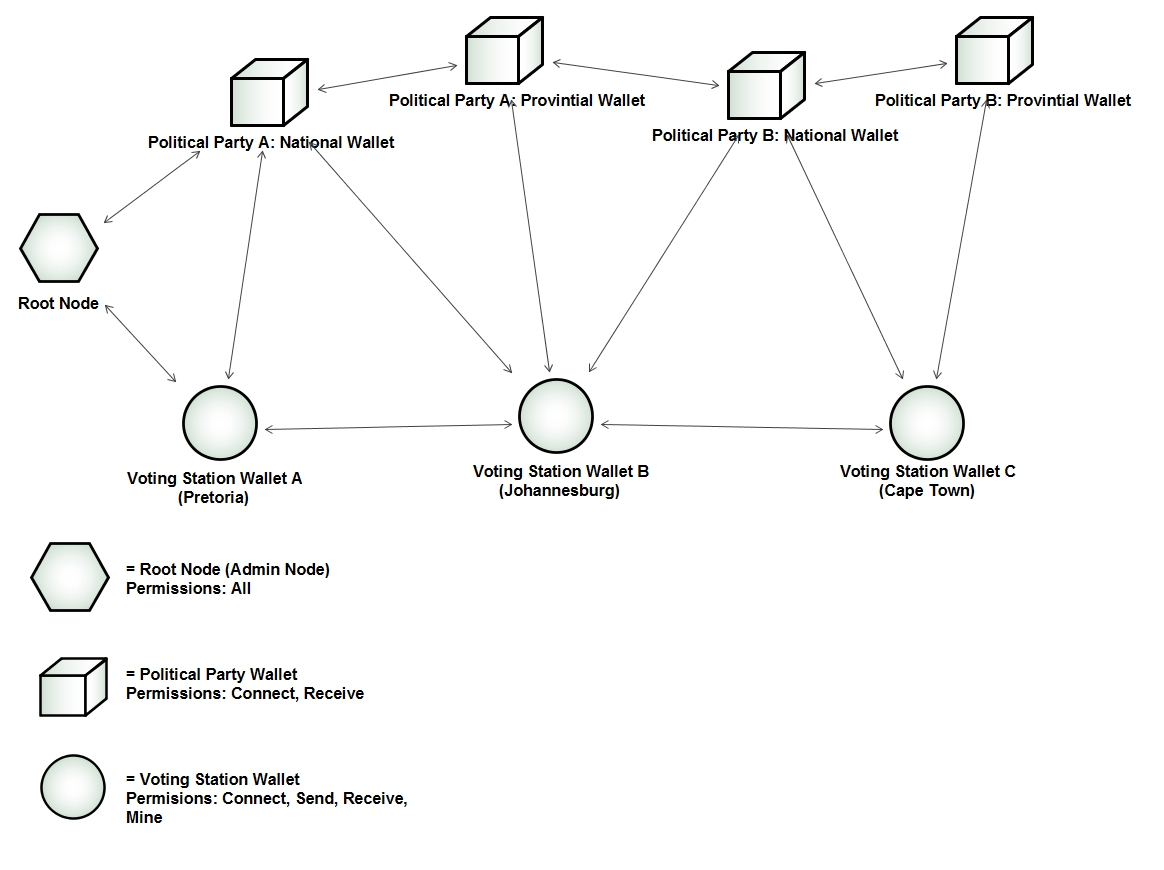
\includegraphics[width=1.25\linewidth]{../Images/UserManual/BlockchainConfiguration1.jpg}
							\caption{Blockchain Node Structure}
							\label{fig:blockchainconfig}
						\end{figure}
						
	TODO may need to elaborate here more
	
	\subsection{Installation}
	TODO: Webservice, database, android app etc
	
	\subsubsection{Blockchain}
	To set up the eVoting Blockchain, each node will need a static IP address.\newline
	Each node will also have a RPC username and RPC password automatically generated by multichain. If however you want to specify custom RPC usernames and RPC password, you may do so, but for the sake of eVoting, the generated RPC password is strong enough.
	
	Each node will require the following setup:
	
	Required Sofware:
	\begin{itemize}
		\item Linux distribution
		\item Multichain. Available at \url{http://www.multichain.com}
	\end{itemize}
	
	System requirements:
	\begin{itemize}
		\item Linux: 64-bit
		\item 512 MB of RAM
		\item 1 GB of disk space.
	\end{itemize}
	
	We chose Lubuntu because it is a minimalist lightweight Linux distribution. Lubuntu is available at \url{http://lubuntu.net/}\newline
	Installation instructions for Multichain can be found at \url{http://www.multichain.com/download-install/}\newline\newline
	
	\paragraph{Setting up a blockchain the Root node}
	
	In the Linux terminal, issue the following commands:\newline\newline
	su [Root-Password]\newline
	multichain-util create EVoting\newline\newline
	You should see the text "Blockchain parameter set was successfully generated."\newline
	The blockchain has been created but isn't running yet, we first need to configure it.\newline
	Edit the "multichain.conf" file at the following default location:\newline
	/root/.multichain/EVoting/multichain.conf\newline
	Here we can specify this node's RPC username and RPC password, but for EVoting we leave it as it is. Then we need to add 2 extra lines to the file, one specifing that this is the Admin Node, the other specifying which network range is allowed to issue remote commands. The file should look something like this (the IP range might need to change in your case):\newline
	rpcuser=multichainrpc\newline
	rpcpassword=Gnb5RsXa783K9LbJGjtfZNpnJg8UbDu8bza8htd9DMPX\newline
	rpcallowip=192.168.43.0/255.255.255.0\newline
	server=1\newline
	rpcport=7419\newline\newline
	
	Then we need to change the actual blockchain configuration. Edit the "params.dat" file and make sure the following values are as follows:\newline\newline\newline
	This part is to ensure the blockchain is private.\newline
	
	anyone-can-connect = false\newline
	anyone-can-send = false\newline
	anyone-can-receive = false\newline
	anyone-can-issue = false\newline
	anyone-can-mine = false\newline
	anyone-can-activate = false\newline
	anyone-can-admin = false\newline
	allow-p2sh-outputs = true\newline
	allow-multisig-outputs = true\newline
	\newline
	The following line is to give the admin an initial value of 10000000 which will be spread between all the Voting Nodes.\newline
	first-block-reward = 1000000\newline\newline
	This line is to make a vote a multiple of 1 and not a decimal value:\newline
	native-currency-multiple = 100000000 \newline\newline
	The complete params.dat file that is used for eVoting can be found on our Github page at EVoting/Documentation/BlockchainConfigurationFiles/params.dat
	\newline\newline
	To start the admin node and also the blockchain, issue the command:\newline
	multichaind EVoting\newline
	Now that the blockchain is running, other nodes can connect to it. In the terminal of the Voting Node, issue this command:\newline
	multichaind EVoting@192.168.1.20:4771\newline
	Where the IP is the IP address of the root node.
\end{document}